\chapter{Introduction}

% \section{Android's Brief History}
% Android is a mobile operating system based on Linux Kernel, developed by Google.
\section{Android's Security Framework}
Android is built on top of Linux Kernel. As with any other UNIX system, the kernel provides drivers for hardware, networking, file-system management, memory management, and process management. However, an Android kernel is slightly different from a "regular" Linux kernel found on a desktop machine. The Android kernel is a stripped down version of the vanilla Linux kernel with some new features (sometimes called Android-isms \cite{yaghmour2013embedded}) that were added to support Android. Some of the most important Android-isms are the low memory killer, wakelocks, ashmen and Binder. Figure \ref{fig:architecture} shows a simplified representation of the Android stack.

\begin{figure}[htb]
\centering
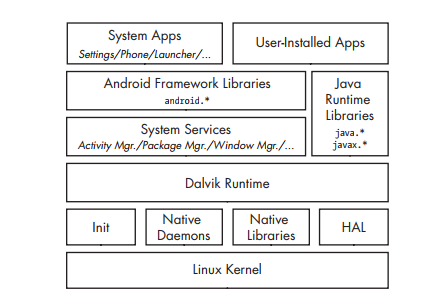
\includegraphics[scale=0.8]{android_architecture.png} % e.g. insert ./image for image.png in the working directory, adjust scale as necessary
\caption{The Android Architecture\cite{Mgr}}
\label{fig:architecture} % insert suitable label, this is used to refer to a fig from within the text as shown above
\end{figure}

Android security model takes advantage of Linux kernel's advanced security features. Linux is a kernel supporting multi-user operating systems, and it can isolate user resources from one another similar to what it does for processes. In Linux, one user cannot access the files of any other user, unless given permissions explicitly and each process runs with the identity of the user (UID and GID) that started it.


Android takes advantage of this user separation mechanism differently. Android was designed to work on mobile devices, and hence there was no need to register different users with the system. Android does not use UID to distinguish users but uses it to distinguish between the applications. This mechanism forms the basis of the Android's application sandboxing. 


\subsection{Android's Application Sandboxing}
Whenever an application is installed, Android automatically assigns a unique UID or app ID and executes that application in a dedicated process running as that UID. Android also creates a dedicated data directory for each application, which only that application has access to read and write to. In this way, Android isolates each application, both at process level by allocating separate process for each application, and at the file level, by allocating private data directory to each application. This mechanism creates a kernel-level application sandbox, which applies to all applications. 

\subsection{Applications}
Applications (or apps) are the programs that users directly interact with. Apps can be divided into user-installed apps and system apps. 

System apps are included in OS image, which is read-only and mounted as /system. These apps cannot be uninstalled or changed by users. Therefore these apps are relatively secure and given more privileges. System apps run under well defined and constant UIDs. Some of the daemons run as the root user also (UID 0). UIDs for system services and applications start from 1000.

User-installed apps are installed on a dedicated read-write partition, typically mounted on /data. This partition stores all the user data and can be uninstalled at will. As mentioned earlier, each application lives in a dedicated sandbox, and typically cannot affect other applications or their data. The user-installed apps can access only those device resources that they have explicitly been granted permission to use. 

\begin{lstlisting}[language=bash,basicstyle=\tiny,caption={Each application process executes as a dedicated user on Android}, captionpos=b, label=listing:sparql_getallindividuals,
   basicstyle=\tiny]
shell@android:/ $ ps
USER    PID   PPID  VSIZE  RSS   WCHAN    PC         NAME
u0_a12  10577 18870 306584 42064 ffffffff 00000000 S com.android.calendar
u0_a21  10594 18870 298804 41164 ffffffff 00000000 S com.android.deskclock
u0_a14  10605 18870 299436 42344 ffffffff 00000000 S com.android.providers.calendar
\end{lstlisting}

The data directory of each application is named after its package name and is created under /data/data/ on single-user devices. All files inside the application's data directory are owned by a dedicated user.
\begin{lstlisting}[language=bash,caption={Application directories are owned by dedicated Linux user}, captionpos=b, label=listing:sparql_getallindividuals, basicstyle=\tiny]
root@android:/ # ls -l /data/data/com.whatsapp/                                
drwxrwx--x u0_a23   u0_a23            2017-10-30 23:53 app_minidumps
drwxrwx--x u0_a23   u0_a23            2017-11-14 00:00 cache
drwx------ u0_a23   u0_a23            2017-10-30 23:53 code_cache
drwxrwx--x u0_a23   u0_a23            2017-11-14 02:01 databases
drwxrwx--x u0_a23   u0_a23            2017-11-14 16:52 files
lrwxrwxrwx install  install           2017-11-13 21:18 lib -> /data/app-lib/com.whatsapp-1
drwx------ u0_a23   u0_a23            2017-10-30 23:53 no_backup
drwxrwx--x u0_a23   u0_a23            2017-11-14 16:52 shared_prefs


\end{lstlisting}

\subsection{Permissions}
Because Android applications are sandboxed in their directories and processes, they can only access their data and any world accessible data on the device. Such limitations largely restrict the applications from providing richer functionality. Hence, Android provides additional, fine-grained access rights to applications so that the applications can use the resources which are not owned by them. These access rights are called permissions. In Android OS, the permissions act as a type of agreement between the user and the app developer. Google, the creator, and maintainer of the OS acts as a moderator between the user and the app developer. It can be described as a three-way relationship between the user, the third-party app developer and Google, which represents the OS. Android OS moderates the relationship between the user and the third-party app developers with the help of the app permissions. Permissions are Android's way of requiring the developers to tell the user how many device resources the app will be using and what information the app will have access to. In Android eco-system, the burden is on the developer to make sure, that the permissions, her app will be using, are informed to the user.


These permissions can control access to device's hardware, network connectivity, and OS services. Applications can request various permissions by listing them in AndroidManifest.xml file. While installing the application, the Android package manager parses this file and asks the user to verify these permissions. Once these permissions are granted, they cannot be revoked, and they are made available to the application without any additional confirmation.

\subsection{SELinux}
The Android security model depends on the UIDs and GIDs assigned to applications. While, by default, this mechanism ensures that each application's files are private, nothing prevents an application from making its files world accessible (intentionally or due to a programming error).

Inappropriate permissions have been the source of many Android vulnerabilities. These vulnerabilities are unavoidable in the default access control model employed by Linux, known as discretionary access control (DAC). In DAC model, once a user gets access to a particular resource, they can pass it on to another user at their discretion.

In contrast, in mandatory access control (MAC) model, a system-wide set of authorized rules called policy are used. MAC ensures that each access to resources conforms to these policies. The policy rules can only be changed by an administrator, and users cannot bypass or override it.

Security Enhanced Linux (SELinux) is a Linux kernel implementation of MAC and has been integrated in the kernel for more than ten years. Android uses a modified SELinux version called the Security Enhancements for Android (SEAndroid).


% \section{Google and Android}

\section{Motivation}
Android is a fairly large and very mature operating system. The constantly increasing number of users and the open source nature of the OS makes it a viable candidate for the best mobile operating system. Study of Security aspects of Android OS provides a good blend of theory (of UNIX principles and security model) and practice. Being open source in nature, it also provides a great opportunity to understand the philosophy of Open Source Software and to get involved in one of largest and most popular open source software, learn about its huge professional code base and interact with the community of developers.